\chapter{System Design}
\label{section:system_design}

\section{High-Level Architecture}

\begin{figure}[H]
    \centering
    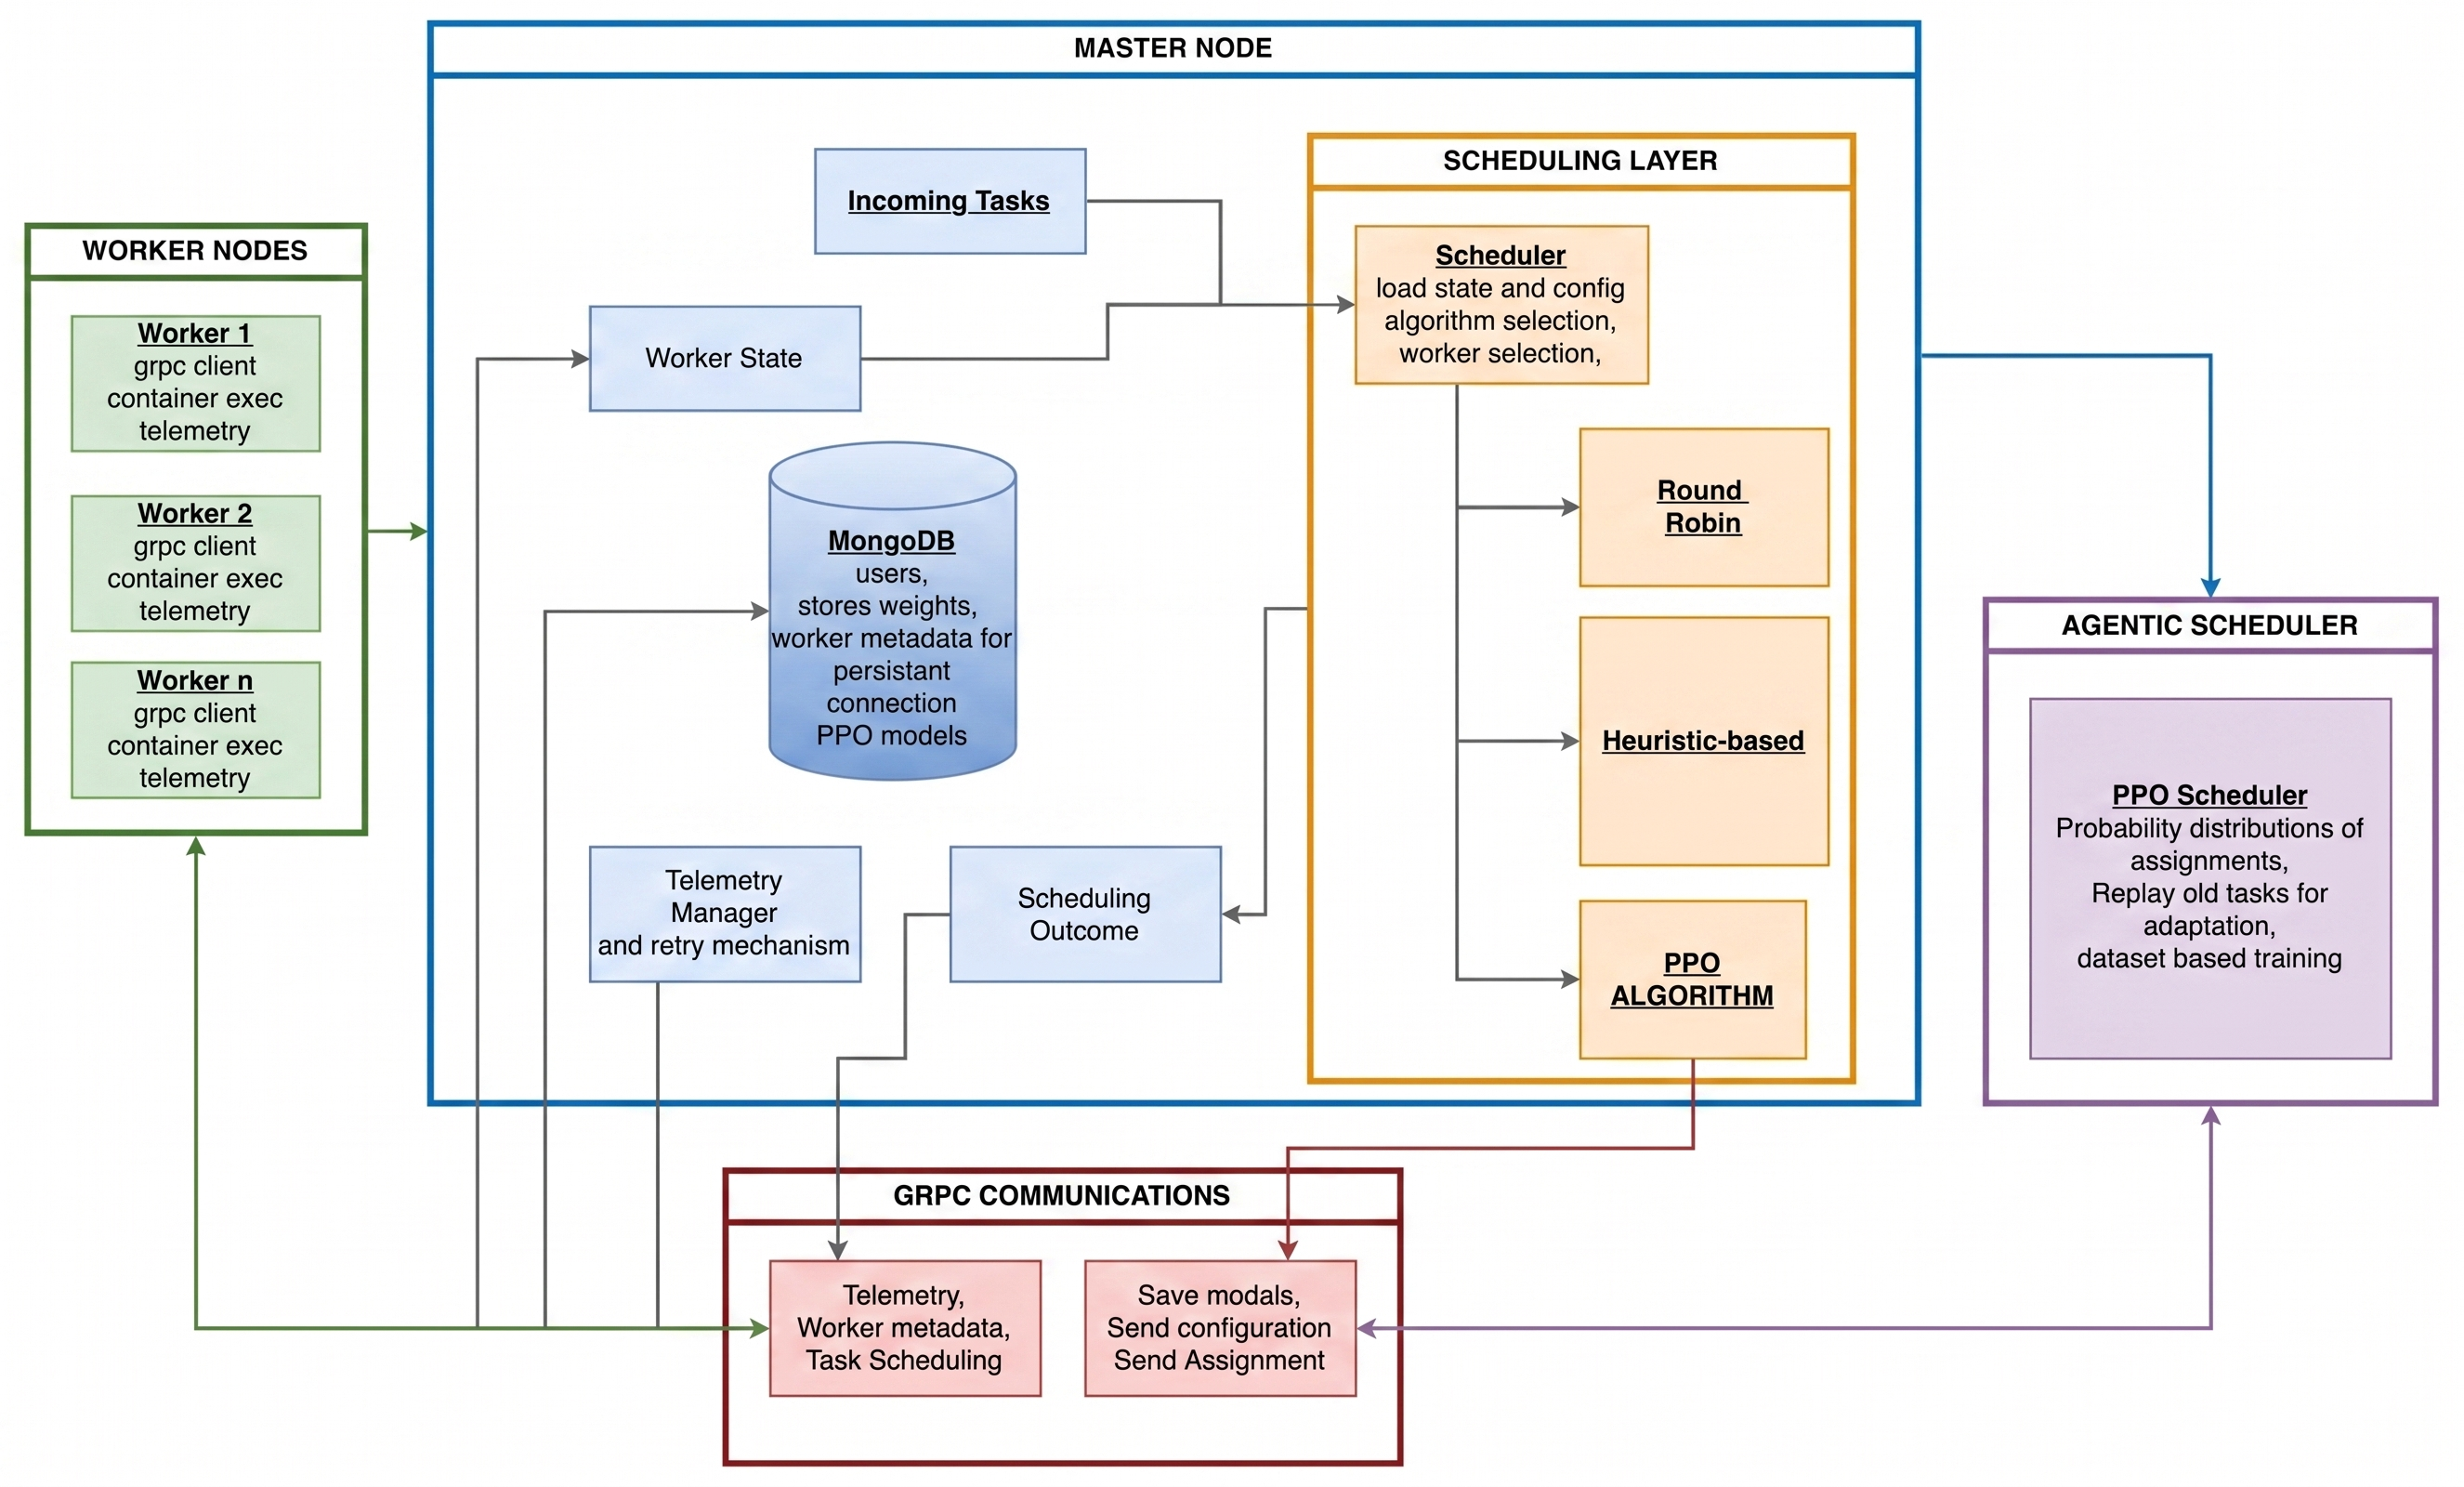
\includegraphics[width=\textwidth]{Figures/Architecture/overall_architecture_colored.png}
    \caption{Overall architecture of Agentic Cloud Cluster}
    \label{fig:overall_architecture}
\end{figure}

\textbf{Explanation of Figure \ref{fig:overall_architecture}:} The system is arranged around a master-worker model. The master node receives task submissions, stores metadata, tracks workers, and calls the scheduler. Worker nodes run the assigned Docker tasks and report status back to the master. The PPO scheduler is separated as a Python service so that the Go control plane stays stable while the learning model can evolve independently.

\section{Go Distributed Cluster Architecture}

The distributed cluster is implemented as a control plane in Go. The design follows a simple rule: the master makes coordination decisions, and workers execute tasks. This keeps the system easy to reason about. A worker does not need to know about other workers. It only needs to accept assignments from the master, execute the container, and report health and task status.

At runtime, the cluster has four main layers:

\begin{enumerate}
    \item \textbf{Client and API layer}: receives task submission and management commands.
    \item \textbf{Master control plane}: validates requests, stores task state, tracks workers, and selects a scheduler.
    \item \textbf{Scheduler layer}: chooses a worker using Round-Robin, RTS, or PPO.
    \item \textbf{Worker execution layer}: runs Docker containers and reports results.
\end{enumerate}

The master and workers communicate using gRPC. The request and response formats are defined in Protocol Buffer files, which keeps communication strict and typed. The master also uses persistent storage for task records, worker metadata, task attempts, and result metadata. The important design point is that scheduling, execution, and persistence are separate modules. This made the project easier to debug because a scheduler bug did not require rewriting the worker executor, and a worker execution bug did not require changing the PPO model.

\section{Master Node}

The master node is the coordinator. Its responsibilities are:

\begin{itemize}
    \item Accept task submissions.
    \item Maintain worker registry and worker health.
    \item Track available CPU, memory, and storage.
    \item Call the active scheduler for each task.
    \item Send task assignments to workers.
    \item Store task state, attempts, and results.
    \item Requeue tasks when workers fail or resources are unavailable.
\end{itemize}

Internally, the master has a few important modules:

\begin{table}[H]
\centering
\caption{Master node modules}
\label{tab:master_modules}
\begin{tabularx}{\textwidth}{lX}
\toprule
\textbf{Module} & \textbf{Role} \\
\midrule
Server layer & Exposes gRPC calls used by workers for registration, heartbeat, task status, and result reporting. \\
Task handling & Creates tasks, tracks state transitions, queues tasks when workers are not available, and records attempts. \\
Worker registry & Maintains active worker IDs, addresses, resource capacities, and current availability. \\
Scheduler package & Provides a common interface for Round-Robin, RTS, and PPO scheduling. \\
Persistence layer & Stores workers, tasks, assignments, attempts, and results. \\
Telemetry manager & Maintains recent worker health and resource state for scheduling and operator inspection. \\
\bottomrule
\end{tabularx}
\end{table}

The scheduler boundary is especially important. The master does not need to know the internal algorithm. It only asks: given this task and these workers, which worker should receive the task? The scheduler returns a worker ID, and the master validates that the worker still exists and still has enough resources before dispatching the task.

\section{Worker Node}

The worker node is responsible for executing tasks. Each worker exposes a gRPC server, accepts assignments from the master, starts a Docker container, tracks execution, streams logs, and reports final status. The worker also sends heartbeat data so the master can maintain a live view of cluster resources.

The worker has three main responsibilities:

\begin{itemize}
    \item \textbf{Registration and heartbeat}: once registered, the worker periodically sends resource and status updates to the master.
    \item \textbf{Container execution}: the worker pulls or uses the requested Docker image, creates the container with the requested resource limits, runs it, and observes the exit code.
    \item \textbf{Result reporting}: after the container exits, the worker reports success or failure and uploads output files if the task produced any.
\end{itemize}

This makes the worker mostly stateless from a cluster point of view. If a worker disappears, the master detects the missed heartbeats and can requeue tasks. The worker does not coordinate with other workers, which avoids complex distributed locking.

\section{Control Flow in the Go Cluster}

The normal task flow is:

\begin{enumerate}
    \item A task is submitted with image name, command, and resource needs.
    \item The master stores the task in created or queued state.
    \item The master builds a live view of feasible workers.
    \item The active scheduler selects a worker.
    \item The master sends the task to that worker through gRPC.
    \item The worker runs the Docker container and streams or records logs.
    \item The worker reports completion.
    \item The master stores the result and releases the worker resources.
\end{enumerate}

The system also supports recovery behavior. If a worker becomes unavailable, the master marks the current attempt as lost and can requeue the logical task. This separation between a logical task and an execution attempt is important because a task may need more than one attempt before it reaches a final state.

\section{Resource Accounting}

Scheduling depends on resource accounting. Each worker advertises total CPU, memory, and storage. The master tracks available resources by subtracting the resources reserved for currently assigned tasks. Once a task completes, those resources are released. This accounting is used both by the simple schedulers and by PPO's action mask.

The design avoids sending tasks to workers that cannot fit them. Even if PPO predicts a worker, the Go master still validates the choice before assignment. This protects the cluster from stale model output or stale worker state.

\section{Task Lifecycle}

\begin{figure}[H]
    \centering
    \begin{tikzpicture}[
        node distance=1.0cm and 0.55cm,
        state/.style={draw=blue!60!black, fill=blue!7, rounded corners, minimum width=3.05cm, minimum height=0.86cm, align=center, font=\small},
        branch/.style={draw=orange!80!black, fill=orange!12, rounded corners, minimum width=3.05cm, minimum height=0.86cm, align=center, font=\small},
        terminal/.style={draw=green!45!black, fill=green!10, rounded corners, minimum width=3.05cm, minimum height=0.86cm, align=center, font=\small},
        fail/.style={draw=red!60!black, fill=red!8, rounded corners, minimum width=3.05cm, minimum height=0.86cm, align=center, font=\small},
        arrow/.style={->, thick}
    ]
        \node[state] (submit) {Task\\Submitted};
        \node[state, right=of submit] (stored0) {Stored\\in Master};
        \node[branch, right=of stored0] (fit) {Feasible\\Worker?};
        \node[state, right=of fit] (select) {Scheduler\\Selects Worker};

        \node[state, below=of select] (assign) {Assignment\\Sent};
        \node[state, left=of assign] (prepare) {Image Pull +\\Container Start};
        \node[state, left=of prepare] (run) {Task\\Running};
        \node[state, left=of run] (monitor) {Logs and\\Exit Code};

        \node[state, below=of monitor] (collect) {Collect\\Output};
        \node[state, right=of collect] (report) {Report\\Result};
        \node[terminal, right=of report] (store) {Store\\Result};
        \node[terminal, right=of store] (success) {Success\\Finish};

        \node[fail, below=of report] (failed) {Failure or\\Lost Worker};
        \node[branch, right=of failed] (retry) {Recoverable\\Failure?};
        \node[state, right=of retry] (requeue) {Requeue as\\New Attempt};
        \node[state, above=0.75cm of fit] (queue) {Wait in\\Queue};

        \draw[arrow] (submit) -- (stored0);
        \draw[arrow] (stored0) -- (fit);
        \draw[arrow] (fit) -- node[above, font=\scriptsize]{yes} (select);
        \draw[arrow] (fit) -- node[left, font=\scriptsize]{no} (queue);
        \draw[arrow] (queue.east) -| (select.north);

        \draw[arrow] (select) -- (assign);
        \draw[arrow] (assign) -- (prepare);
        \draw[arrow] (prepare) -- (run);
        \draw[arrow] (run) -- (monitor);

        \draw[arrow] (monitor) -- (collect);
        \draw[arrow] (collect) -- (report);
        \draw[arrow] (report) -- (store);
        \draw[arrow] (store) -- (success);
        \draw[arrow] (report) -- (failed);

        \draw[arrow] (failed) -- (retry);
        \draw[arrow] (retry) -- node[above, font=\scriptsize]{yes} (requeue);
        \draw[arrow] (retry.north) |- node[pos=0.25, right, font=\scriptsize]{no} (store.south);
    \end{tikzpicture}
    \caption{Task lifecycle in the cluster}
    \label{fig:task_lifecycle}
\end{figure}

\textbf{Explanation of Figure \ref{fig:task_lifecycle}:} The lifecycle is shown as a grid so that each state is readable. A task starts when it is submitted and stored by the master. The master checks whether at least one worker can fit the task. If no worker is feasible, the task waits in the queue and is checked again later. If a worker is feasible, the scheduler selects a worker, the assignment is sent, and the worker prepares the Docker container. After execution, the worker reports logs, exit status, and output files. The master stores the result. A successful task finishes, while a recoverable failure can be requeued as a new attempt.

\section{Task Execution Flow}

\begin{figure}[H]
    \centering
    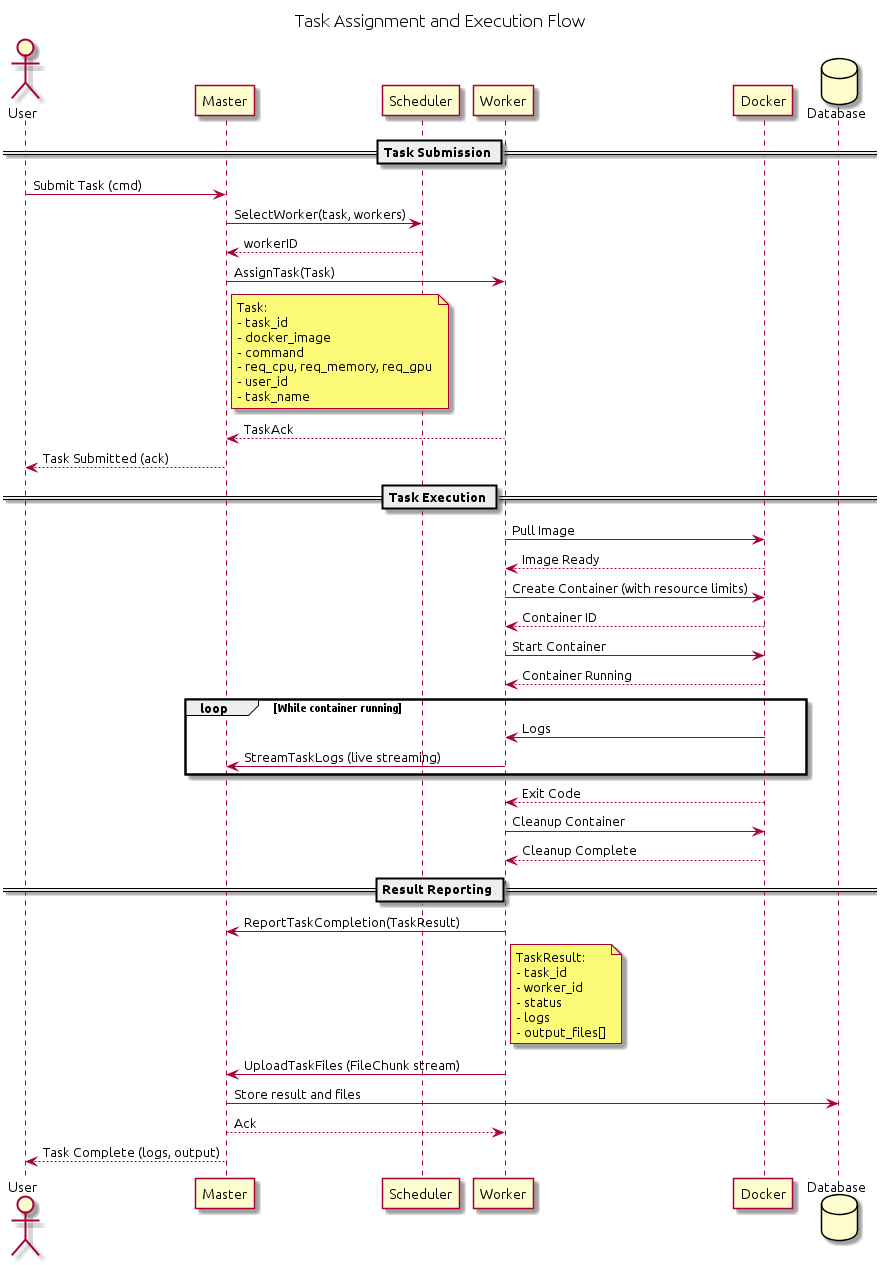
\includegraphics[height=0.78\textheight]{Figures/Architecture/task_execution.png}
    \caption{Task assignment and execution flow}
    \label{fig:task_execution}
\end{figure}

\textbf{Explanation of Figure \ref{fig:task_execution}:} The master first receives a task and asks the scheduler to choose a worker. The assignment is sent to the worker through gRPC. The worker runs the Docker container and reports completion. The design keeps the scheduling decision separate from execution, which made it possible to compare Round-Robin, heuristic scheduling, and PPO without rewriting the worker.

\section{Scheduler Interface}

The scheduler receives:

\begin{itemize}
    \item task CPU requirement,
    \item task memory requirement,
    \item task storage requirement,
    \item task type,
    \item worker capacity,
    \item worker availability,
    \item worker activity status.
\end{itemize}

It returns a worker ID. This simple interface allowed the project to start with baselines and later add PPO. The PPO scheduler calls a Python service over gRPC. If the PPO service is unavailable or returns an unsuitable worker, the Go scheduler falls back to a safer scheduler. This was a deliberate design decision because a learning model should improve scheduling, not make the whole cluster fragile.

\section{PPO Deployment Design}

The PPO deployment supports three modes:

\begin{table}[H]
\centering
\caption{PPO deployment modes}
\label{tab:ppo_modes}
\begin{tabularx}{\textwidth}{lX}
\toprule
\textbf{Mode} & \textbf{Meaning} \\
\midrule
Active & PPO makes the scheduling decision, with fallback on failure. \\
Shadow & PPO is queried for comparison, but the fallback scheduler is used for the actual placement. \\
Fallback & PPO is bypassed and the fallback scheduler is used directly. \\
\bottomrule
\end{tabularx}
\end{table}

This design was chosen because model deployment in systems work must be conservative. The system can test PPO decisions without immediately trusting them in production paths.
